\documentclass[a4paper,10pt]{article}
\usepackage[utf8]{inputenc}
\usepackage{graphicx}

%opening
\title{Tracing Aufg 11.2}
\author{Can Nayci, Leonhard Rattmann, Emil Sharaf}

\begin{document}

\maketitle

Randnotiz: Die Ausführung des Programms mit Score-P sorgt für Probleme, wie u.a. auch schon bei GS 3/2 (Ende) zu sehen. Daher wurden für die restliche Analyse die Traces von Patricks Gruppe geliehen.

\section{Startphase}
Auf den Ausschnitten ist nicht abgebildet, wie die Verschiedenen Prozesse zu unterschiedlichen Zeiten \textit{MPI\_Init} starten. Womöglich liegt das an dem Hyperthreading; die ersten zwei Prozesse lägen dabei auf z.B. HW-Core 0 usw..

Bei GS 3/2 sieht man klar, wie $p_0$ zuerst seine Berechnung macht, $p_1$ damit freigibt usw., also das Treppenmodell ähnlich dem Konzept. Da JA 3/2

Im anderen Modell wird nach \textit{MPI\_Init} erst das options-struct per Broadcast verschickt (da askParams bei allen Prozessen läuft wäre das optional)
\begin{figure}
  \caption{Startphase GS 3/2}
  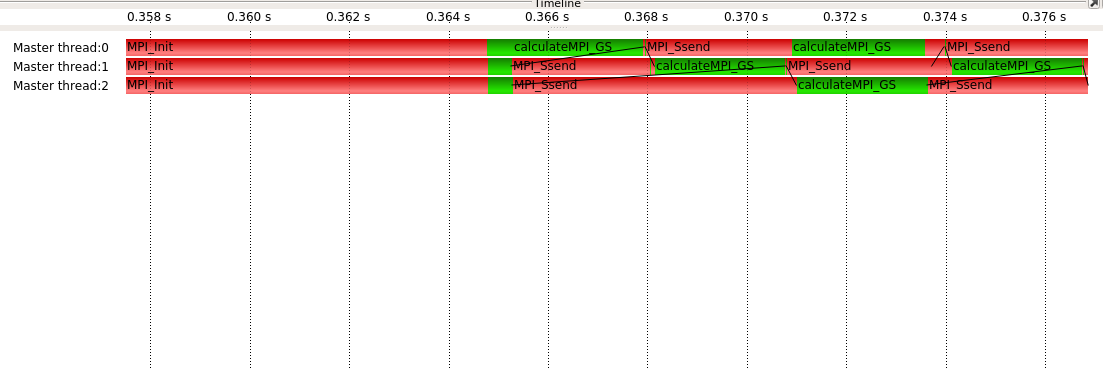
\includegraphics[width=14cm]{c_start_GS_3x2.png}
\end{figure}
\begin{figure}
  \caption{Startphase JA 3/2}
  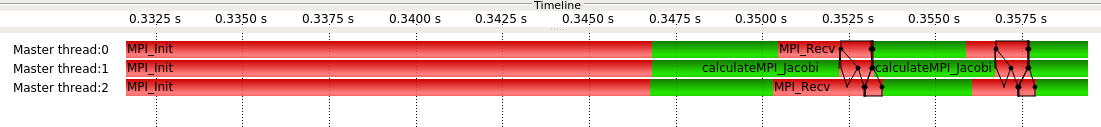
\includegraphics[width=14cm]{c_start_JA_3x2.png}
\end{figure}
\begin{figure}
  \caption{Startphase GS 3/2 (Patrick)}
  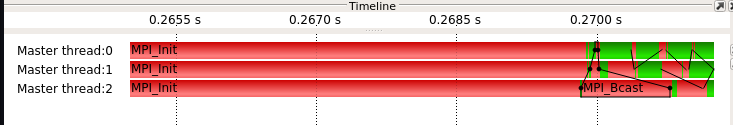
\includegraphics[width=14cm]{Patrick/c_start_GS_3x2.png}
\end{figure}
\begin{figure}
  \caption{Startphase JA 3/2 (Patrick)}
  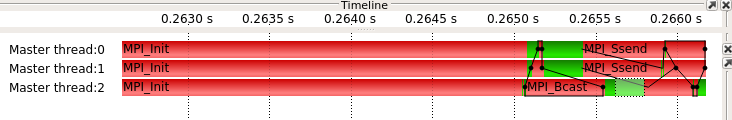
\includegraphics[width=14cm]{Patrick/c_start_JA_3x2.png}
\end{figure}
\begin{figure}
  \caption{Startphase GS 5/4 (Patrick)}
  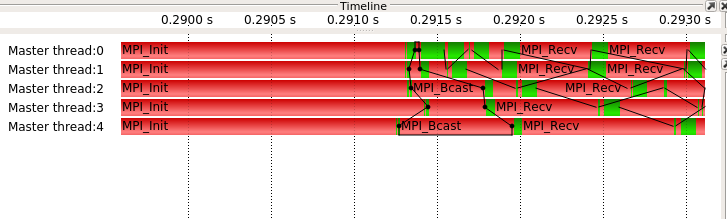
\includegraphics[width=14cm]{Patrick/c_start_GS_5x4.png}
\end{figure}
\section{Synchronisation}
\begin{figure}
 \caption{Synchronisation GS 3/2}
 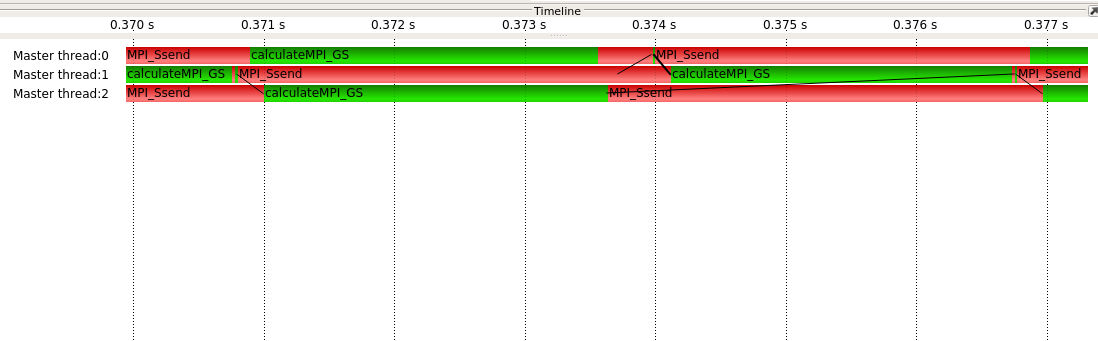
\includegraphics[width=14cm]{c_sync_GS_3x2.png}
\end{figure}
\begin{figure}
 \caption{Synchronisation JA 3/2}
 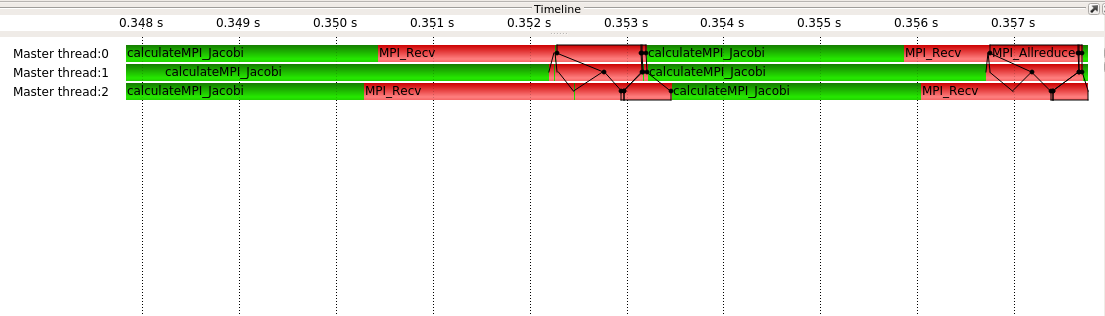
\includegraphics[width=14cm]{c_sync_JA_3x2.png}
\end{figure}
\section{Endphase}
\begin{figure}
 \caption{Endphase GS 3/2}
 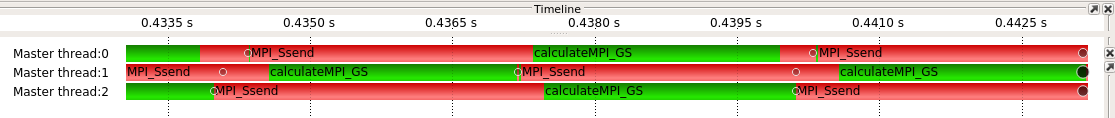
\includegraphics[width=14cm]{c_end_GS_3x2.png}
\end{figure}
\begin{figure}
 \caption{Endphase JA 3/2}
 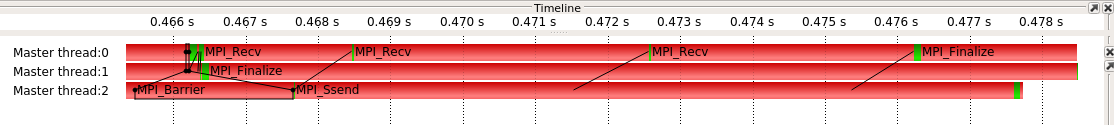
\includegraphics[width=14cm]{c_end_JA_3x2.png}
\end{figure}

\end{document}
